% Appendix fragment: experiment 2 -- the information is never encoded.
% Included from main.tex via % Appendix fragment: experiment 2 -- the information is never encoded.
% Included from main.tex via % Appendix fragment: experiment 2 -- the information is never encoded.
% Included from main.tex via % Appendix fragment: experiment 2 -- the information is never encoded.
% Included from main.tex via \input{appendix_encoding}; uses the macros defined there.

\section{The information is never encoded}\label{app:encoding}

\paragraph{Protocol.} An item is a \emph{certified encoding failure} when it is wrong under the
uniform bar and right under the oracle crop at the same budget; this is the label no other work can
construct, because it needs the crop control. The layer-wise read-out is a logit lens: intermediate
layers are decoded as $\mathrm{lm\_head}(\mathrm{final\_norm}(h_\ell))$, while the final layer is
read from the model's own logits, because applying the final norm to the last hidden state as well
double-normalises that layer alone and corrupted an earlier result of ours (\S\ref{app:mech}); we
assert per run that the last-layer read-out matches the true logits. Representation patching replaces
the image tokens' hidden states at a single layer's output with those of a donor image carrying the
same question at the same token budget; the pre-registered controls are that patching the image at
L4 must be large and patching text at L20 must be large.

\paragraph{The answer is not in the stack.} If the answer were present but mis-routed, a layer-wise
read-out would find it somewhere and lose it later. Under the uniform encoding no layer's decoded
answer exceeds $52.9\%$, and localisation quality does not change that: on items where the window
covers the target and the model still answers wrong ($n{=}36$), the correct option is the argmax at
some layer on $72.2\%$ of items, against $68.1\%$ where the window missed entirely. There is no
layer at which the answer is present and subsequently lost: the apparent signal at L20 ($41.7\%$)
collapses to $0\%$ from L22 and matches what near-chance layers produce by chance. Under the oracle
crop the lens instead reaches $92.6\%$, and the answer appears abruptly at L22, taking $90\%$ of the
gain in a single transition; the step replicates one layer later on Qwen2-VL-7B and appears only
where the crop covers the target ($+23.8$ points covered, exactly $0.0$ where it misses). Cropping
does not make the model reason better; it supplies information that a fixed depth converts into an
answer. Representation patching agrees from the other side: replacing every image token's hidden
state with a different image's, at a single layer, changes the answer no more than replacing
irrelevant early text once past the transport boundary (KL $0.009$ vs $0.009$ on Qwen3 and $0.005$
vs $0.006$ on Qwen2 at L16). The oracle crop fixes $94.4\%$ of the localised-but-wrong items at the
same budget, with a median of $0.14$ merged tokens on target, and across the benchmark
$37.7\%$/$41.4\%$ of all items are certified encoding failures: $86.7\%$/$84.0\%$ of every error,
rising to $94.0\%$/$89.4\%$ at $W{=}0.15$.

\begin{figure}[h]\centering
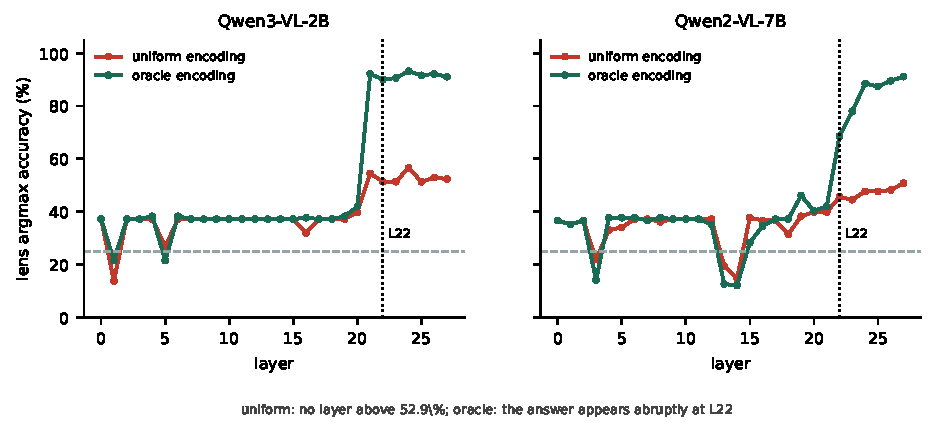
\includegraphics[width=\textwidth]{figs/fig_lens.pdf}
\caption{\textbf{The answer is not in the stack.} Per-layer logit-lens accuracy under the uniform
encoding (red) and the oracle crop (green), both models. Uniform: flat, no layer above $52.9\%$ and
none holding an answer that is later lost. Oracle: the answer becomes decodable abruptly at L22,
taking most of the gain in one transition; the Qwen2 step is one layer later.}
\label{fig:lens}
\end{figure}

\paragraph{Why the target is invisible.} The arithmetic behind the threshold is simple. At the
$300$-token pass the median single-region target's side is $0.210$ merged tokens; $100\%$ of targets
are smaller than one merged token, the median target occupies $0.176$ tokens of area, and $62\%$ sit
below the $0.25$-token cliff. The evidence is averaged into a single token's footprint together with
its background before the language model ever sees it --- which is why magnification, not budget, is
the operation that recovers it.

\begin{figure}[h]\centering
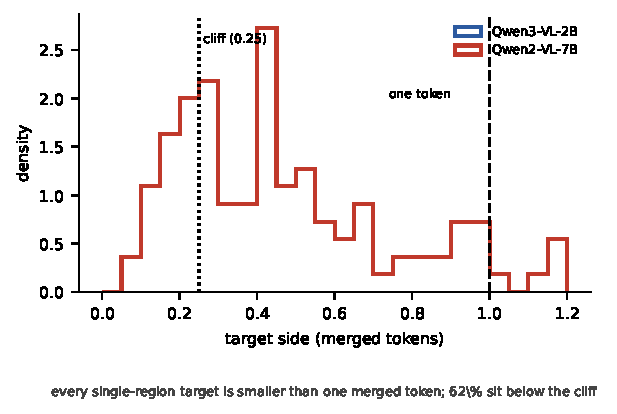
\includegraphics[width=0.62\textwidth]{figs/fig_footprint.pdf}
\caption{\textbf{The target is smaller than a token.} Distribution of the single-region target's side
in merged-token units at the $300$-token pass, both models. Every target lies left of the one-token
line; most lie below the $0.25$-token cliff.}
\label{fig:footprint}
\end{figure}

\paragraph{Controls.} Two further controls bound the interpretation. \emph{Localisation degrades
below the cliff, far less than accuracy}: ground-truth coverage falls from $0.637$ to $0.457$
(argmax window) and from $0.751$ to $0.580$ (head window) on Qwen3, and $0.594\to0.450$ /
$0.620\to0.471$ on Qwen2, while accuracy falls by $42.6$ points --- encoding dominates, placement
contributes a minority share. \emph{The below-chance failure is not the language prior}: a text-only
control (question without the image) agrees with the image-conditioned answer on $49.4\%$ of
below-cliff items vs $40.7\%$ above on Qwen3, but $49.4\%$ vs $56.5\%$ on Qwen2 --- opposite
directions, neither interval clear. Below the cliff the model is systematically misled, but not by
the text-only prior.
; uses the macros defined there.

\section{The information is never encoded}\label{app:encoding}

\paragraph{Protocol.} An item is a \emph{certified encoding failure} when it is wrong under the
uniform bar and right under the oracle crop at the same budget; this is the label no other work can
construct, because it needs the crop control. The layer-wise read-out is a logit lens: intermediate
layers are decoded as $\mathrm{lm\_head}(\mathrm{final\_norm}(h_\ell))$, while the final layer is
read from the model's own logits, because applying the final norm to the last hidden state as well
double-normalises that layer alone and corrupted an earlier result of ours (\S\ref{app:mech}); we
assert per run that the last-layer read-out matches the true logits. Representation patching replaces
the image tokens' hidden states at a single layer's output with those of a donor image carrying the
same question at the same token budget; the pre-registered controls are that patching the image at
L4 must be large and patching text at L20 must be large.

\paragraph{The answer is not in the stack.} If the answer were present but mis-routed, a layer-wise
read-out would find it somewhere and lose it later. Under the uniform encoding no layer's decoded
answer exceeds $52.9\%$, and localisation quality does not change that: on items where the window
covers the target and the model still answers wrong ($n{=}36$), the correct option is the argmax at
some layer on $72.2\%$ of items, against $68.1\%$ where the window missed entirely. There is no
layer at which the answer is present and subsequently lost: the apparent signal at L20 ($41.7\%$)
collapses to $0\%$ from L22 and matches what near-chance layers produce by chance. Under the oracle
crop the lens instead reaches $92.6\%$, and the answer appears abruptly at L22, taking $90\%$ of the
gain in a single transition; the step replicates one layer later on Qwen2-VL-7B and appears only
where the crop covers the target ($+23.8$ points covered, exactly $0.0$ where it misses). Cropping
does not make the model reason better; it supplies information that a fixed depth converts into an
answer. Representation patching agrees from the other side: replacing every image token's hidden
state with a different image's, at a single layer, changes the answer no more than replacing
irrelevant early text once past the transport boundary (KL $0.009$ vs $0.009$ on Qwen3 and $0.005$
vs $0.006$ on Qwen2 at L16). The oracle crop fixes $94.4\%$ of the localised-but-wrong items at the
same budget, with a median of $0.14$ merged tokens on target, and across the benchmark
$37.7\%$/$41.4\%$ of all items are certified encoding failures: $86.7\%$/$84.0\%$ of every error,
rising to $94.0\%$/$89.4\%$ at $W{=}0.15$.

\begin{figure}[h]\centering
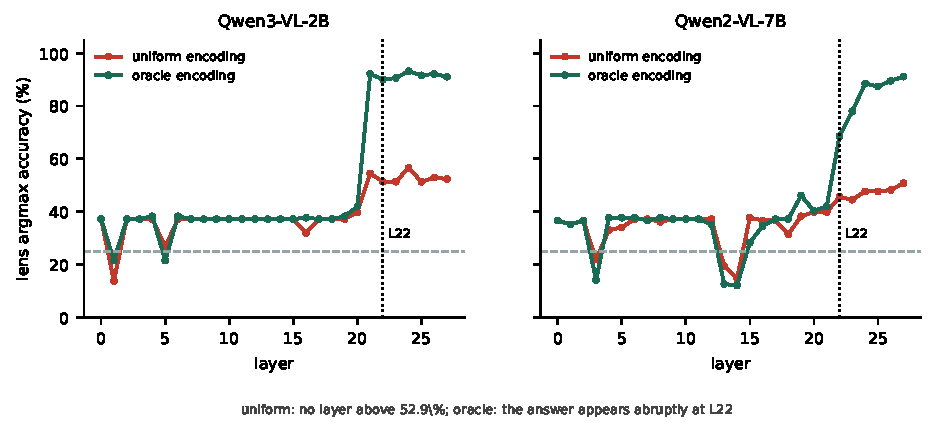
\includegraphics[width=\textwidth]{figs/fig_lens.pdf}
\caption{\textbf{The answer is not in the stack.} Per-layer logit-lens accuracy under the uniform
encoding (red) and the oracle crop (green), both models. Uniform: flat, no layer above $52.9\%$ and
none holding an answer that is later lost. Oracle: the answer becomes decodable abruptly at L22,
taking most of the gain in one transition; the Qwen2 step is one layer later.}
\label{fig:lens}
\end{figure}

\paragraph{Why the target is invisible.} The arithmetic behind the threshold is simple. At the
$300$-token pass the median single-region target's side is $0.210$ merged tokens; $100\%$ of targets
are smaller than one merged token, the median target occupies $0.176$ tokens of area, and $62\%$ sit
below the $0.25$-token cliff. The evidence is averaged into a single token's footprint together with
its background before the language model ever sees it --- which is why magnification, not budget, is
the operation that recovers it.

\begin{figure}[h]\centering
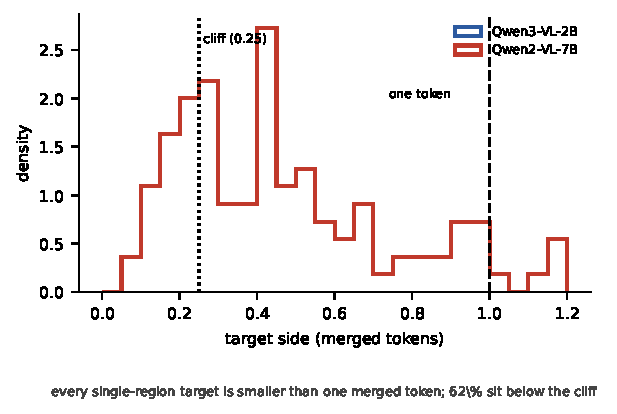
\includegraphics[width=0.62\textwidth]{figs/fig_footprint.pdf}
\caption{\textbf{The target is smaller than a token.} Distribution of the single-region target's side
in merged-token units at the $300$-token pass, both models. Every target lies left of the one-token
line; most lie below the $0.25$-token cliff.}
\label{fig:footprint}
\end{figure}

\paragraph{Controls.} Two further controls bound the interpretation. \emph{Localisation degrades
below the cliff, far less than accuracy}: ground-truth coverage falls from $0.637$ to $0.457$
(argmax window) and from $0.751$ to $0.580$ (head window) on Qwen3, and $0.594\to0.450$ /
$0.620\to0.471$ on Qwen2, while accuracy falls by $42.6$ points --- encoding dominates, placement
contributes a minority share. \emph{The below-chance failure is not the language prior}: a text-only
control (question without the image) agrees with the image-conditioned answer on $49.4\%$ of
below-cliff items vs $40.7\%$ above on Qwen3, but $49.4\%$ vs $56.5\%$ on Qwen2 --- opposite
directions, neither interval clear. Below the cliff the model is systematically misled, but not by
the text-only prior.
; uses the macros defined there.

\section{The information is never encoded}\label{app:encoding}

\paragraph{Protocol.} An item is a \emph{certified encoding failure} when it is wrong under the
uniform bar and right under the oracle crop at the same budget; this is the label no other work can
construct, because it needs the crop control. The layer-wise read-out is a logit lens: intermediate
layers are decoded as $\mathrm{lm\_head}(\mathrm{final\_norm}(h_\ell))$, while the final layer is
read from the model's own logits, because applying the final norm to the last hidden state as well
double-normalises that layer alone and corrupted an earlier result of ours (\S\ref{app:mech}); we
assert per run that the last-layer read-out matches the true logits. Representation patching replaces
the image tokens' hidden states at a single layer's output with those of a donor image carrying the
same question at the same token budget; the pre-registered controls are that patching the image at
L4 must be large and patching text at L20 must be large.

\paragraph{The answer is not in the stack.} If the answer were present but mis-routed, a layer-wise
read-out would find it somewhere and lose it later. Under the uniform encoding no layer's decoded
answer exceeds $52.9\%$, and localisation quality does not change that: on items where the window
covers the target and the model still answers wrong ($n{=}36$), the correct option is the argmax at
some layer on $72.2\%$ of items, against $68.1\%$ where the window missed entirely. There is no
layer at which the answer is present and subsequently lost: the apparent signal at L20 ($41.7\%$)
collapses to $0\%$ from L22 and matches what near-chance layers produce by chance. Under the oracle
crop the lens instead reaches $92.6\%$, and the answer appears abruptly at L22, taking $90\%$ of the
gain in a single transition; the step replicates one layer later on Qwen2-VL-7B and appears only
where the crop covers the target ($+23.8$ points covered, exactly $0.0$ where it misses). Cropping
does not make the model reason better; it supplies information that a fixed depth converts into an
answer. Representation patching agrees from the other side: replacing every image token's hidden
state with a different image's, at a single layer, changes the answer no more than replacing
irrelevant early text once past the transport boundary (KL $0.009$ vs $0.009$ on Qwen3 and $0.005$
vs $0.006$ on Qwen2 at L16). The oracle crop fixes $94.4\%$ of the localised-but-wrong items at the
same budget, with a median of $0.14$ merged tokens on target, and across the benchmark
$37.7\%$/$41.4\%$ of all items are certified encoding failures: $86.7\%$/$84.0\%$ of every error,
rising to $94.0\%$/$89.4\%$ at $W{=}0.15$.

\begin{figure}[h]\centering
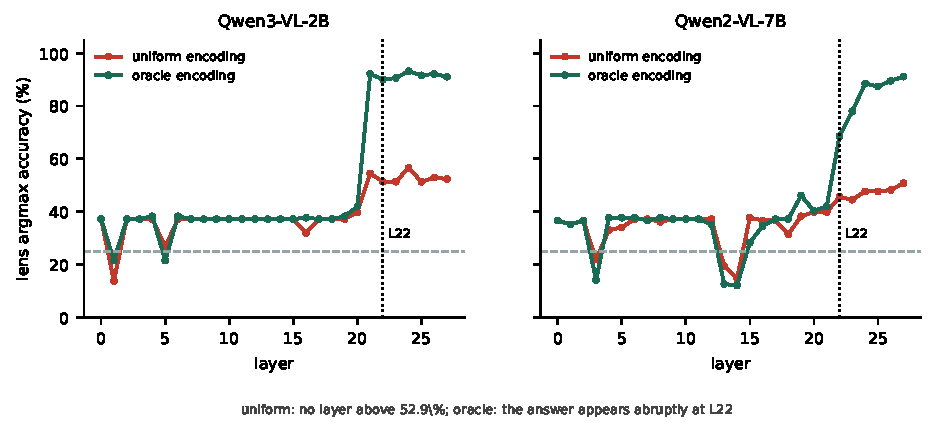
\includegraphics[width=\textwidth]{figs/fig_lens.pdf}
\caption{\textbf{The answer is not in the stack.} Per-layer logit-lens accuracy under the uniform
encoding (red) and the oracle crop (green), both models. Uniform: flat, no layer above $52.9\%$ and
none holding an answer that is later lost. Oracle: the answer becomes decodable abruptly at L22,
taking most of the gain in one transition; the Qwen2 step is one layer later.}
\label{fig:lens}
\end{figure}

\paragraph{Why the target is invisible.} The arithmetic behind the threshold is simple. At the
$300$-token pass the median single-region target's side is $0.210$ merged tokens; $100\%$ of targets
are smaller than one merged token, the median target occupies $0.176$ tokens of area, and $62\%$ sit
below the $0.25$-token cliff. The evidence is averaged into a single token's footprint together with
its background before the language model ever sees it --- which is why magnification, not budget, is
the operation that recovers it.

\begin{figure}[h]\centering
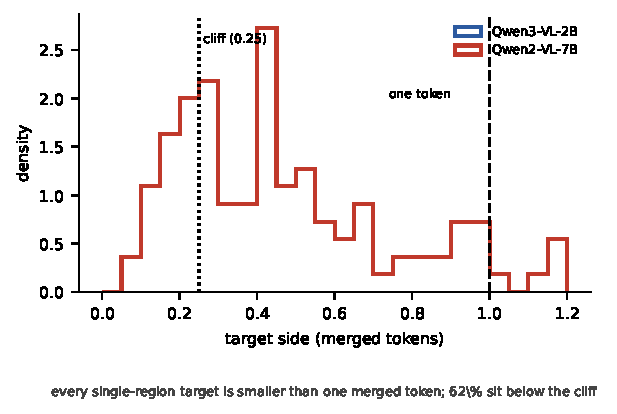
\includegraphics[width=0.62\textwidth]{figs/fig_footprint.pdf}
\caption{\textbf{The target is smaller than a token.} Distribution of the single-region target's side
in merged-token units at the $300$-token pass, both models. Every target lies left of the one-token
line; most lie below the $0.25$-token cliff.}
\label{fig:footprint}
\end{figure}

\paragraph{Controls.} Two further controls bound the interpretation. \emph{Localisation degrades
below the cliff, far less than accuracy}: ground-truth coverage falls from $0.637$ to $0.457$
(argmax window) and from $0.751$ to $0.580$ (head window) on Qwen3, and $0.594\to0.450$ /
$0.620\to0.471$ on Qwen2, while accuracy falls by $42.6$ points --- encoding dominates, placement
contributes a minority share. \emph{The below-chance failure is not the language prior}: a text-only
control (question without the image) agrees with the image-conditioned answer on $49.4\%$ of
below-cliff items vs $40.7\%$ above on Qwen3, but $49.4\%$ vs $56.5\%$ on Qwen2 --- opposite
directions, neither interval clear. Below the cliff the model is systematically misled, but not by
the text-only prior.
; uses the macros defined there.

\section{The information is never encoded}\label{app:encoding}

\paragraph{Protocol.} An item is a \emph{certified encoding failure} when it is wrong under the
uniform bar and right under the oracle crop at the same budget; this is the label no other work can
construct, because it needs the crop control. The layer-wise read-out is a logit lens: intermediate
layers are decoded as $\mathrm{lm\_head}(\mathrm{final\_norm}(h_\ell))$, while the final layer is
read from the model's own logits, because applying the final norm to the last hidden state as well
double-normalises that layer alone and corrupted an earlier result of ours (\S\ref{app:mech}); we
assert per run that the last-layer read-out matches the true logits. Representation patching replaces
the image tokens' hidden states at a single layer's output with those of a donor image carrying the
same question at the same token budget; the pre-registered controls are that patching the image at
L4 must be large and patching text at L20 must be large.

\paragraph{The answer is not in the stack.} If the answer were present but mis-routed, a layer-wise
read-out would find it somewhere and lose it later. Under the uniform encoding no layer's decoded
answer exceeds $52.9\%$, and localisation quality does not change that: on items where the window
covers the target and the model still answers wrong ($n{=}36$), the correct option is the argmax at
some layer on $72.2\%$ of items, against $68.1\%$ where the window missed entirely. There is no
layer at which the answer is present and subsequently lost: the apparent signal at L20 ($41.7\%$)
collapses to $0\%$ from L22 and matches what near-chance layers produce by chance. Under the oracle
crop the lens instead reaches $92.6\%$, and the answer appears abruptly at L22, taking $90\%$ of the
gain in a single transition; the step replicates one layer later on Qwen2-VL-7B and appears only
where the crop covers the target ($+23.8$ points covered, exactly $0.0$ where it misses). Cropping
does not make the model reason better; it supplies information that a fixed depth converts into an
answer. Representation patching agrees from the other side: replacing every image token's hidden
state with a different image's, at a single layer, changes the answer no more than replacing
irrelevant early text once past the transport boundary (KL $0.009$ vs $0.009$ on Qwen3 and $0.005$
vs $0.006$ on Qwen2 at L16). The oracle crop fixes $94.4\%$ of the localised-but-wrong items at the
same budget, with a median of $0.14$ merged tokens on target, and across the benchmark
$37.7\%$/$41.4\%$ of all items are certified encoding failures: $86.7\%$/$84.0\%$ of every error,
rising to $94.0\%$/$89.4\%$ at $W{=}0.15$.

\begin{figure}[h]\centering
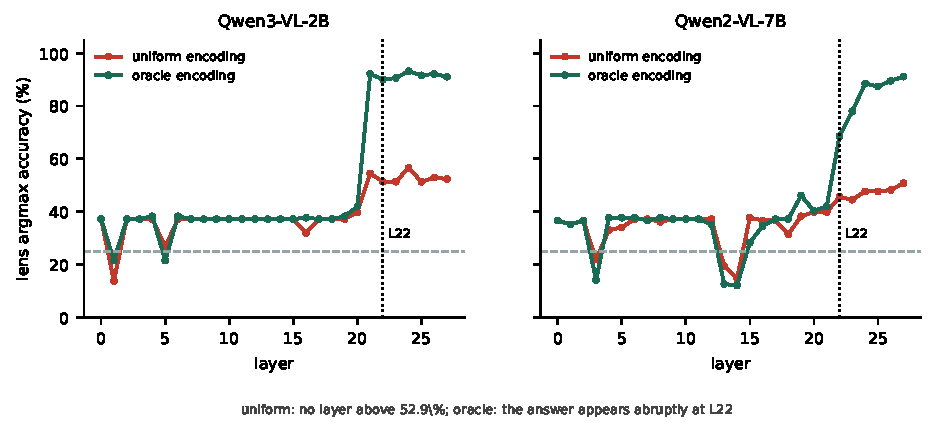
\includegraphics[width=\textwidth]{figs/fig_lens.pdf}
\caption{\textbf{The answer is not in the stack.} Per-layer logit-lens accuracy under the uniform
encoding (red) and the oracle crop (green), both models. Uniform: flat, no layer above $52.9\%$ and
none holding an answer that is later lost. Oracle: the answer becomes decodable abruptly at L22,
taking most of the gain in one transition; the Qwen2 step is one layer later.}
\label{fig:lens}
\end{figure}

\paragraph{Why the target is invisible.} The arithmetic behind the threshold is simple. At the
$300$-token pass the median single-region target's side is $0.210$ merged tokens; $100\%$ of targets
are smaller than one merged token, the median target occupies $0.176$ tokens of area, and $62\%$ sit
below the $0.25$-token cliff. The evidence is averaged into a single token's footprint together with
its background before the language model ever sees it --- which is why magnification, not budget, is
the operation that recovers it.

\begin{figure}[h]\centering
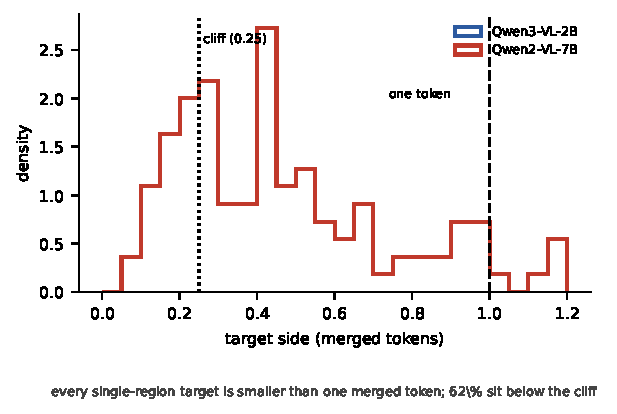
\includegraphics[width=0.62\textwidth]{figs/fig_footprint.pdf}
\caption{\textbf{The target is smaller than a token.} Distribution of the single-region target's side
in merged-token units at the $300$-token pass, both models. Every target lies left of the one-token
line; most lie below the $0.25$-token cliff.}
\label{fig:footprint}
\end{figure}

\paragraph{Controls.} Two further controls bound the interpretation. \emph{Localisation degrades
below the cliff, far less than accuracy}: ground-truth coverage falls from $0.637$ to $0.457$
(argmax window) and from $0.751$ to $0.580$ (head window) on Qwen3, and $0.594\to0.450$ /
$0.620\to0.471$ on Qwen2, while accuracy falls by $42.6$ points --- encoding dominates, placement
contributes a minority share. \emph{The below-chance failure is not the language prior}: a text-only
control (question without the image) agrees with the image-conditioned answer on $49.4\%$ of
below-cliff items vs $40.7\%$ above on Qwen3, but $49.4\%$ vs $56.5\%$ on Qwen2 --- opposite
directions, neither interval clear. Below the cliff the model is systematically misled, but not by
the text-only prior.
